%!TEX root = ../thesis.tex
% ******************************* Thesis Appendix B ********************************

\chapter{}
\ifpdf
\graphicspath{{chapter-simplify/Figs/Raster/}{chapter-simplify/Figs/PDF/}{chapter-simplify/Figs/}}
\else
\graphicspath{{chapter-simplify/Figs/Vector/}{chapter-simplify/Figs/}}
\fi

\section{Simplified likelihood results}

\begin{figure}
\floatbox[{\capbeside\thisfloatsetup{capbesideposition={right,center},capbesidewidth=0.35\textwidth}}]{figure}[\FBwidth]
{\caption{Comparison of the simplified likelihood (blue contours) and full likelihood (orange contours) results for the search for electroweakinos presented previously. The observed contours are shown as solid lines, while the expected contours are shown as dashed lines. Observed CL$_s$ values from both likelihoods are given. The uncertainty band includes all \gls{mc} statistical and systematic uncertainties in the case of the full likelihood, and only the simplified uncertainties in the case of the simplified likelihood.}\label{fig:app_results_simplify_1Lbb}}
{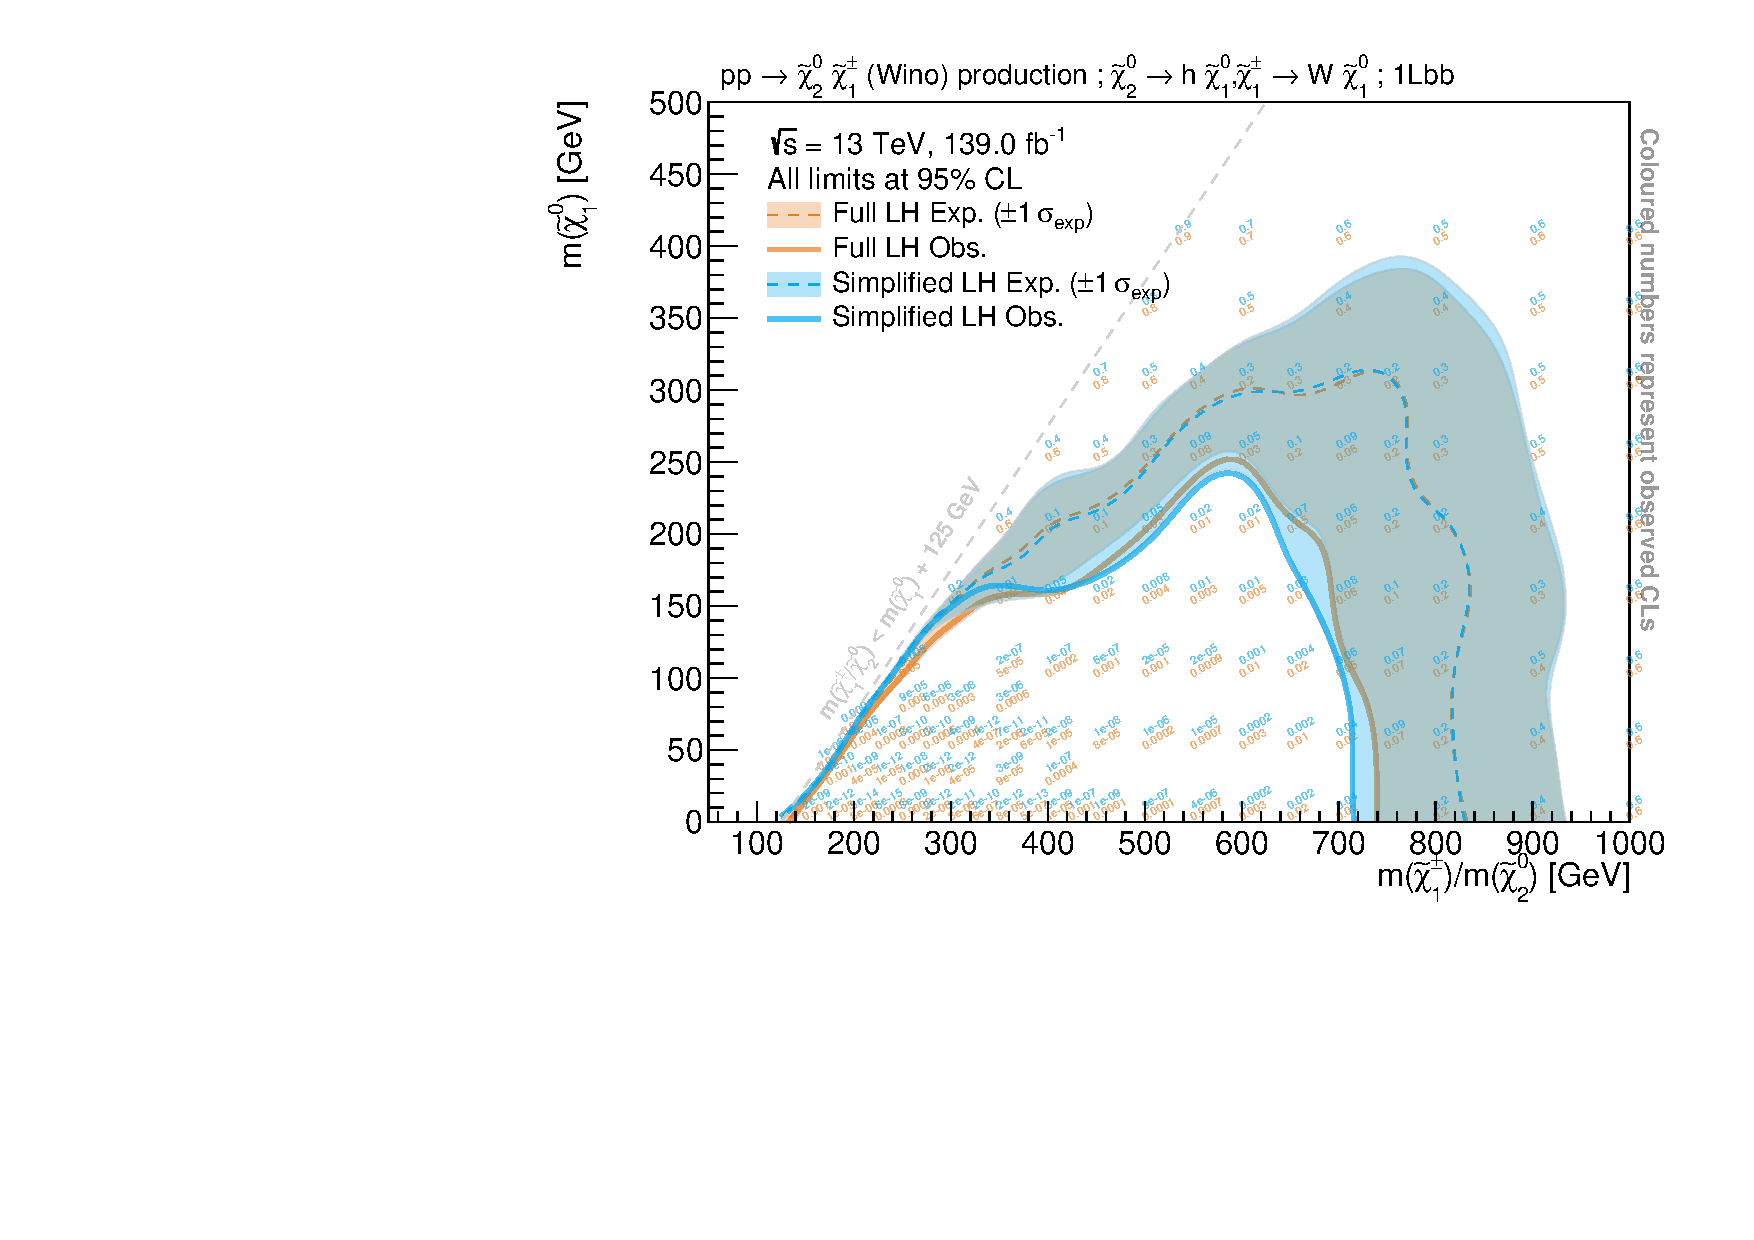
\includegraphics[width=0.60\textwidth]{exclusion_1Lbb_CLs_noLabel}}
\end{figure}



\begin{figure}
	\centering
	\begin{subfigure}[b]{0.5\textwidth}
		\centering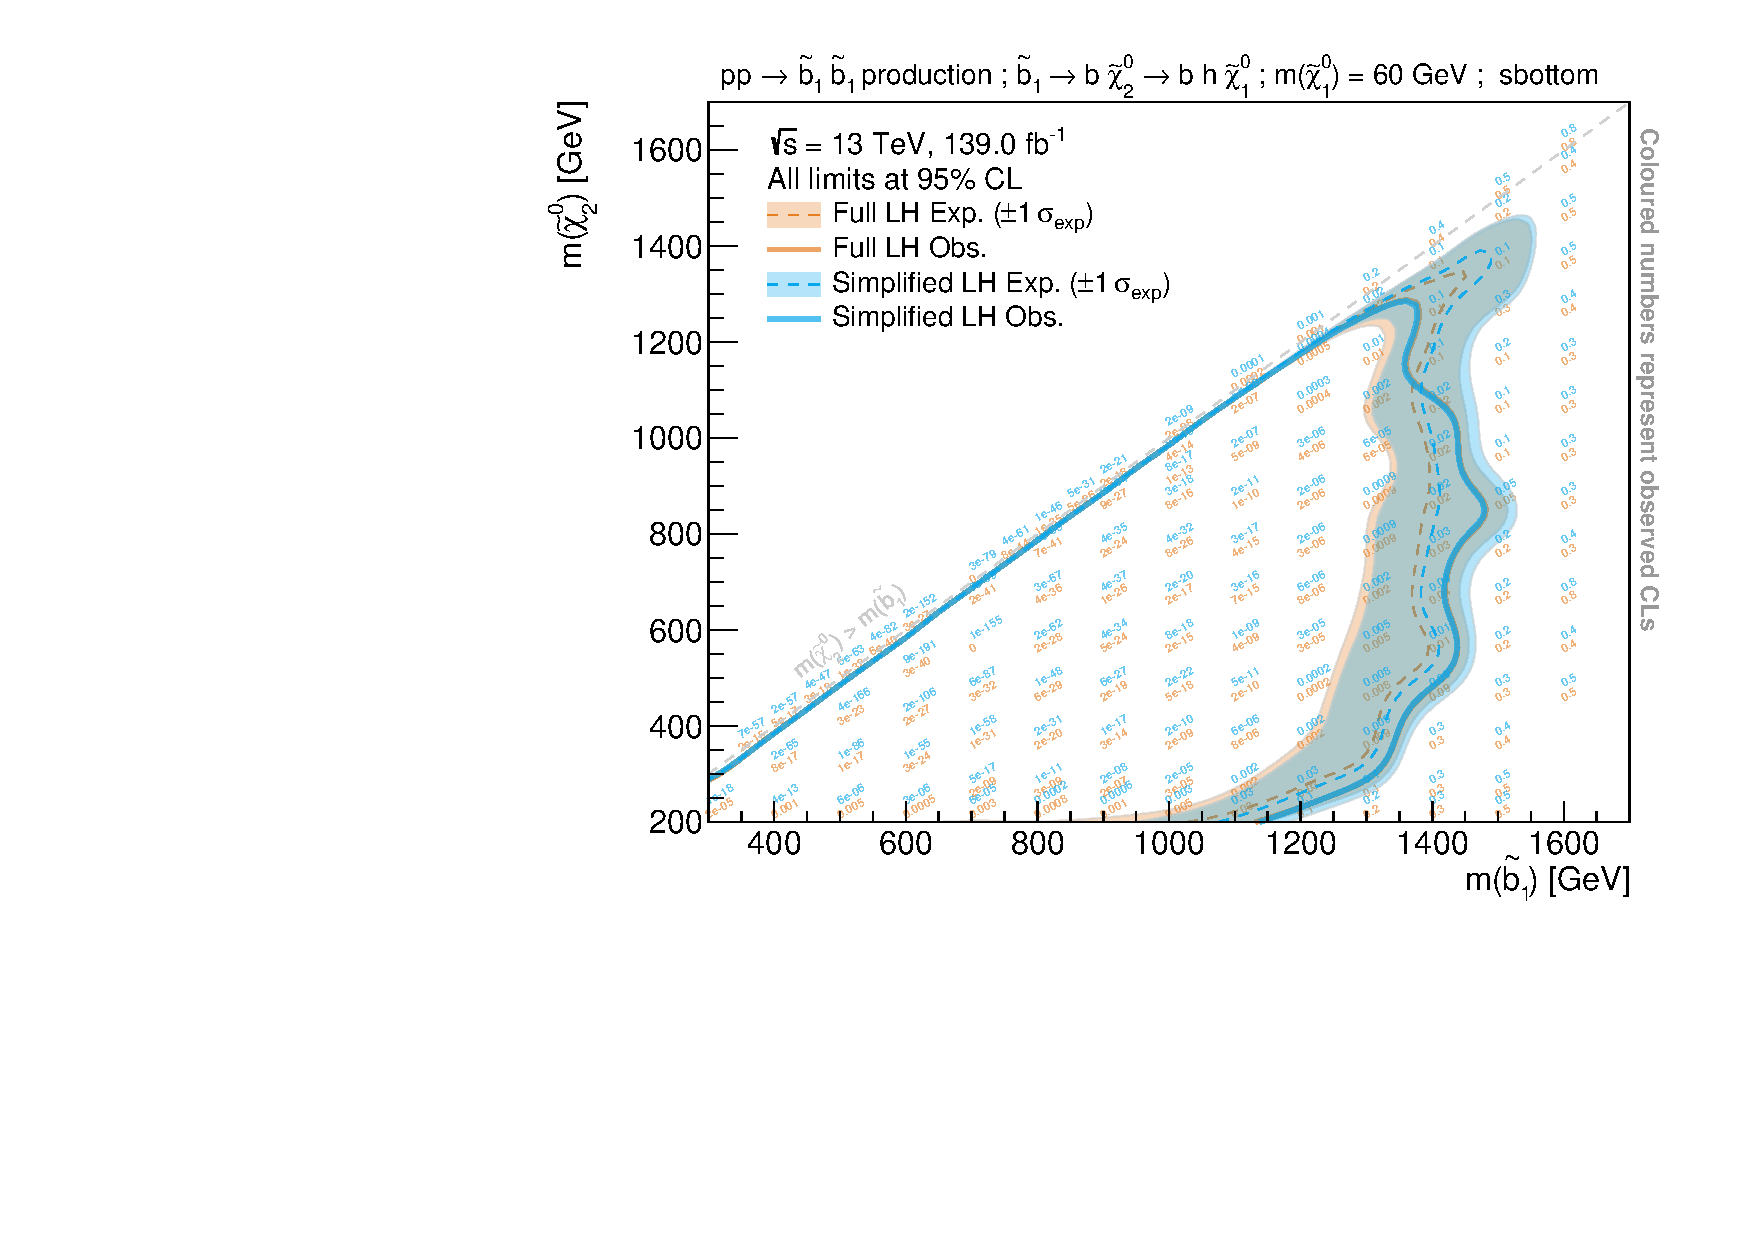
\includegraphics[width=\textwidth]{exclusion_sbottom_CLs_noLabel}
		\caption{ATLAS sbottom search~\cite{SUSY-2018-31}\label{fig:results_sbottom}}
	\end{subfigure}\hfill
	\begin{subfigure}[b]{0.5\textwidth}
		\centering\includegraphics[width=\textwidth]{exclusion_stop1L_CLs_noLabel}
		\caption{ATLAS stop search\label{fig:results_stop1L}}
	\end{subfigure}\hfill
	\begin{subfigure}[b]{0.5\textwidth}
		\centering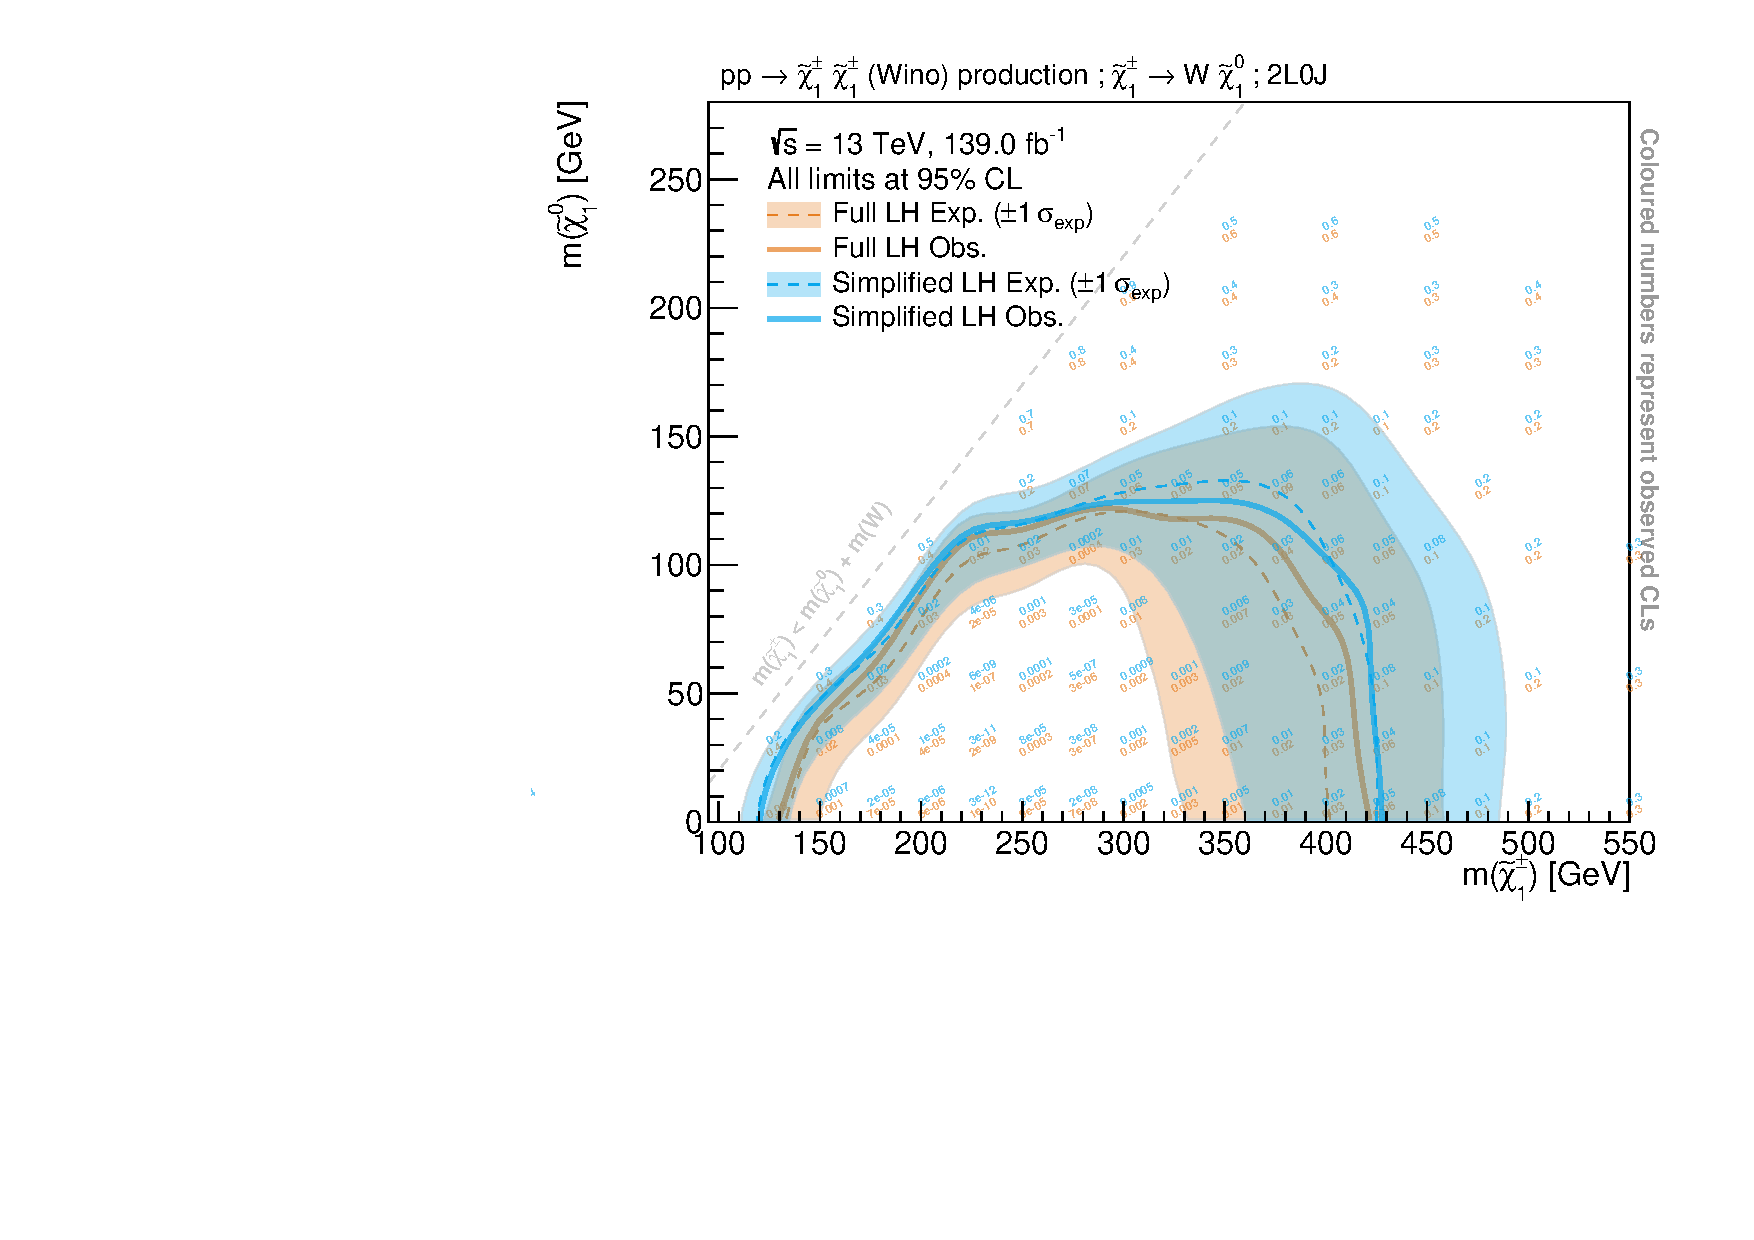
\includegraphics[width=\textwidth]{exclusion_2L0J_CLs_noLabel}
		\caption{ATLAS 2-lepton search~\cite{SUSY-2018-32}\label{fig:results_2L0J}}
	\end{subfigure}\hfill
	\begin{subfigure}[b]{0.5\textwidth}
		\centering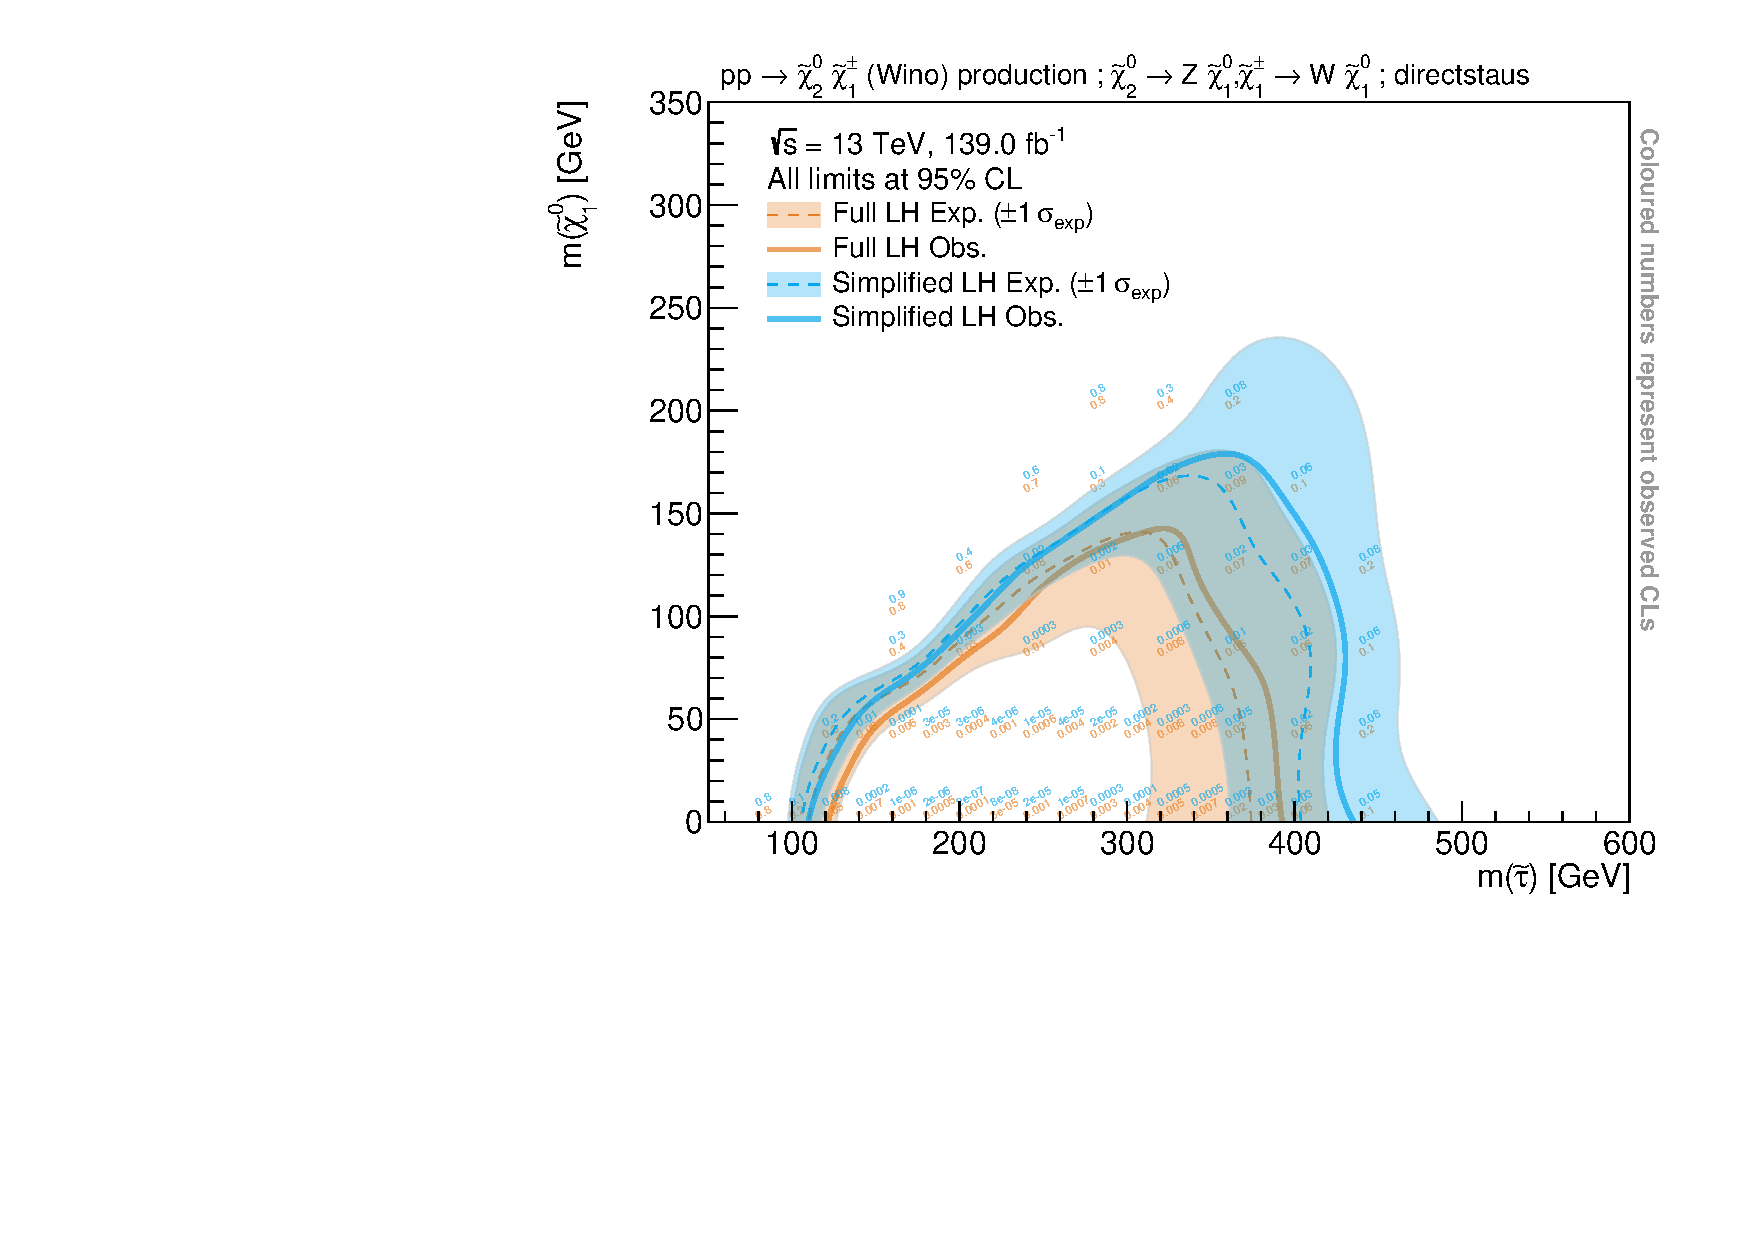
\includegraphics[width=\textwidth]{exclusion_directstaus_CLs_noLabel}
		\caption{ATLAS direct stau search~\cite{SUSY-2018-04}\label{fig:results_directstaus}}
	\end{subfigure}\hfill
	\begin{subfigure}[b]{0.5\textwidth}
		\centering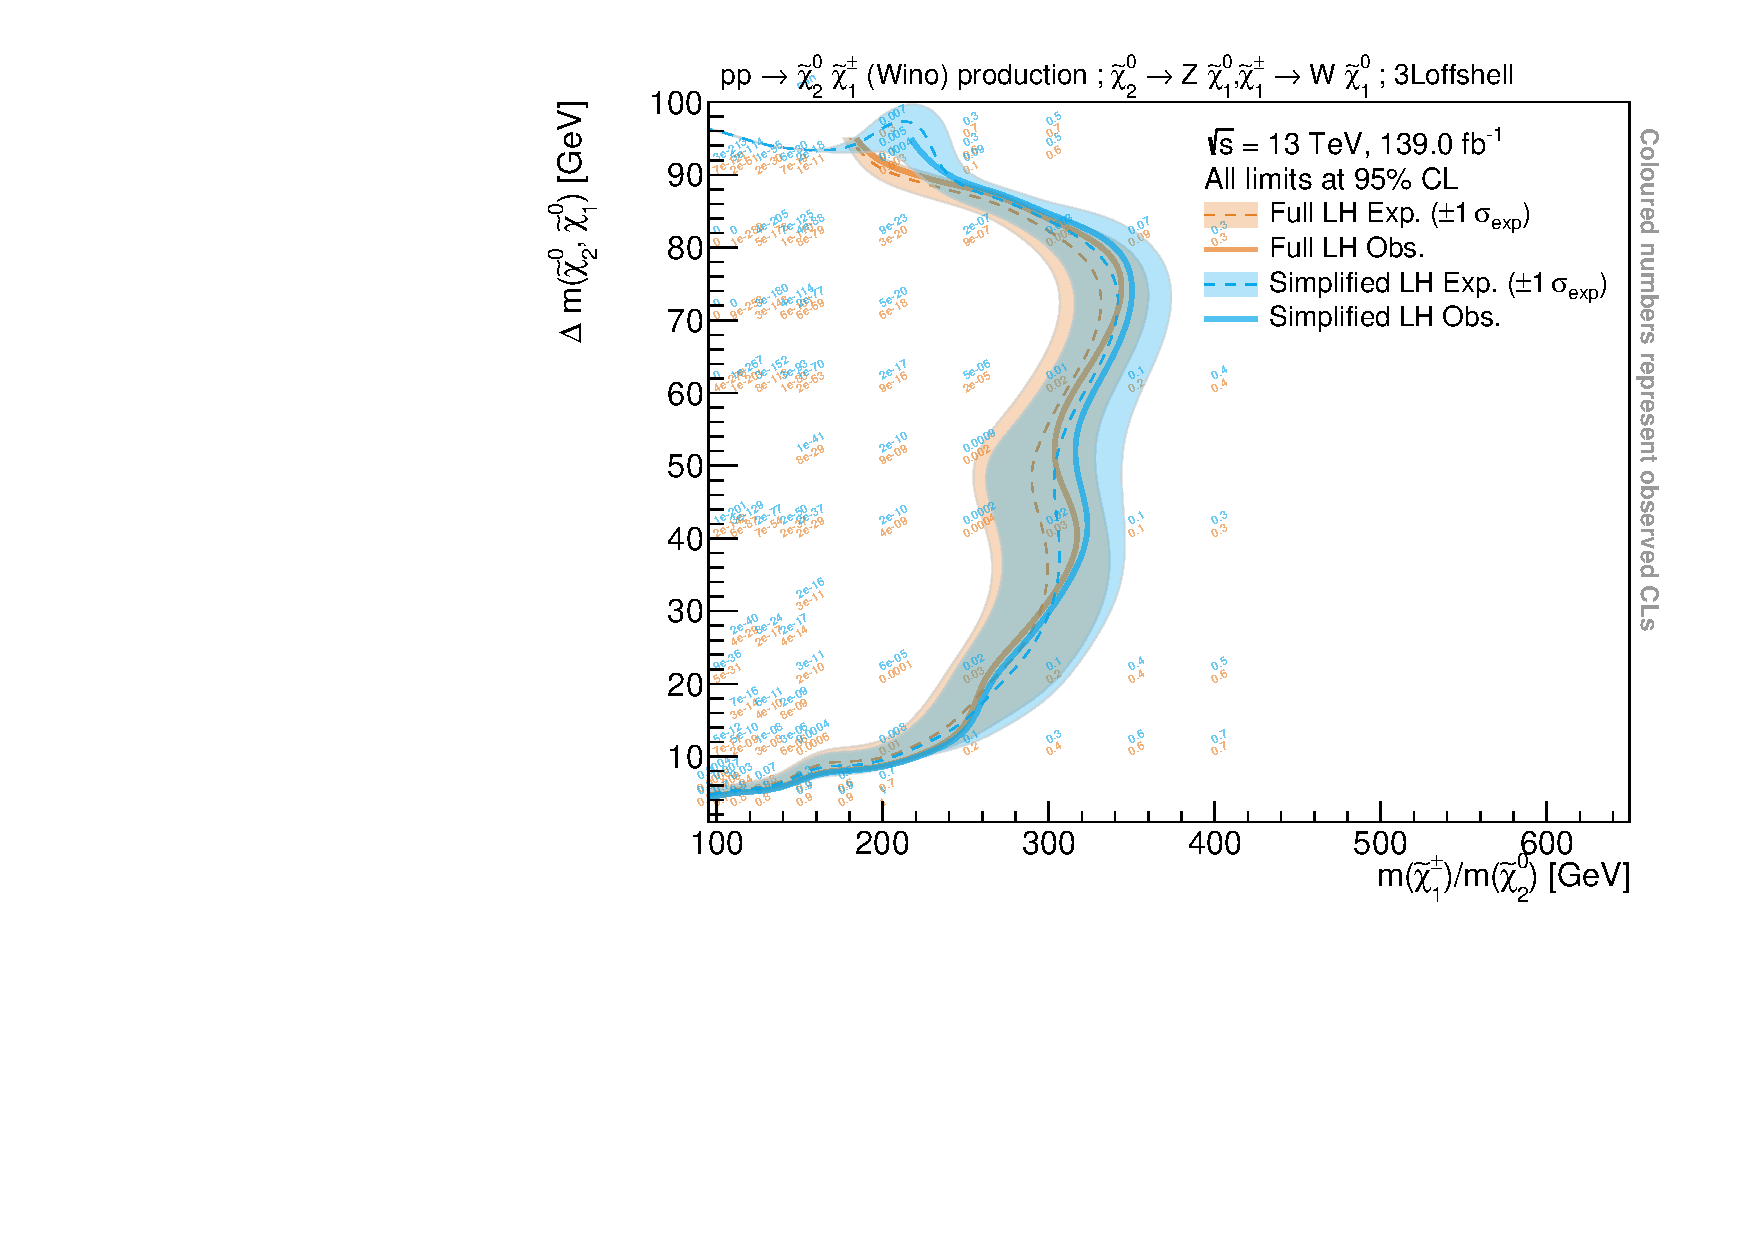
\includegraphics[width=\textwidth]{exclusion_3Loffshell_CLs_noLabel}
		\caption{ATLAS 3-lepton search\label{fig:results_3Loffshell}}
	\end{subfigure}\hfill
	\begin{subfigure}[b]{0.5\textwidth}
		\centering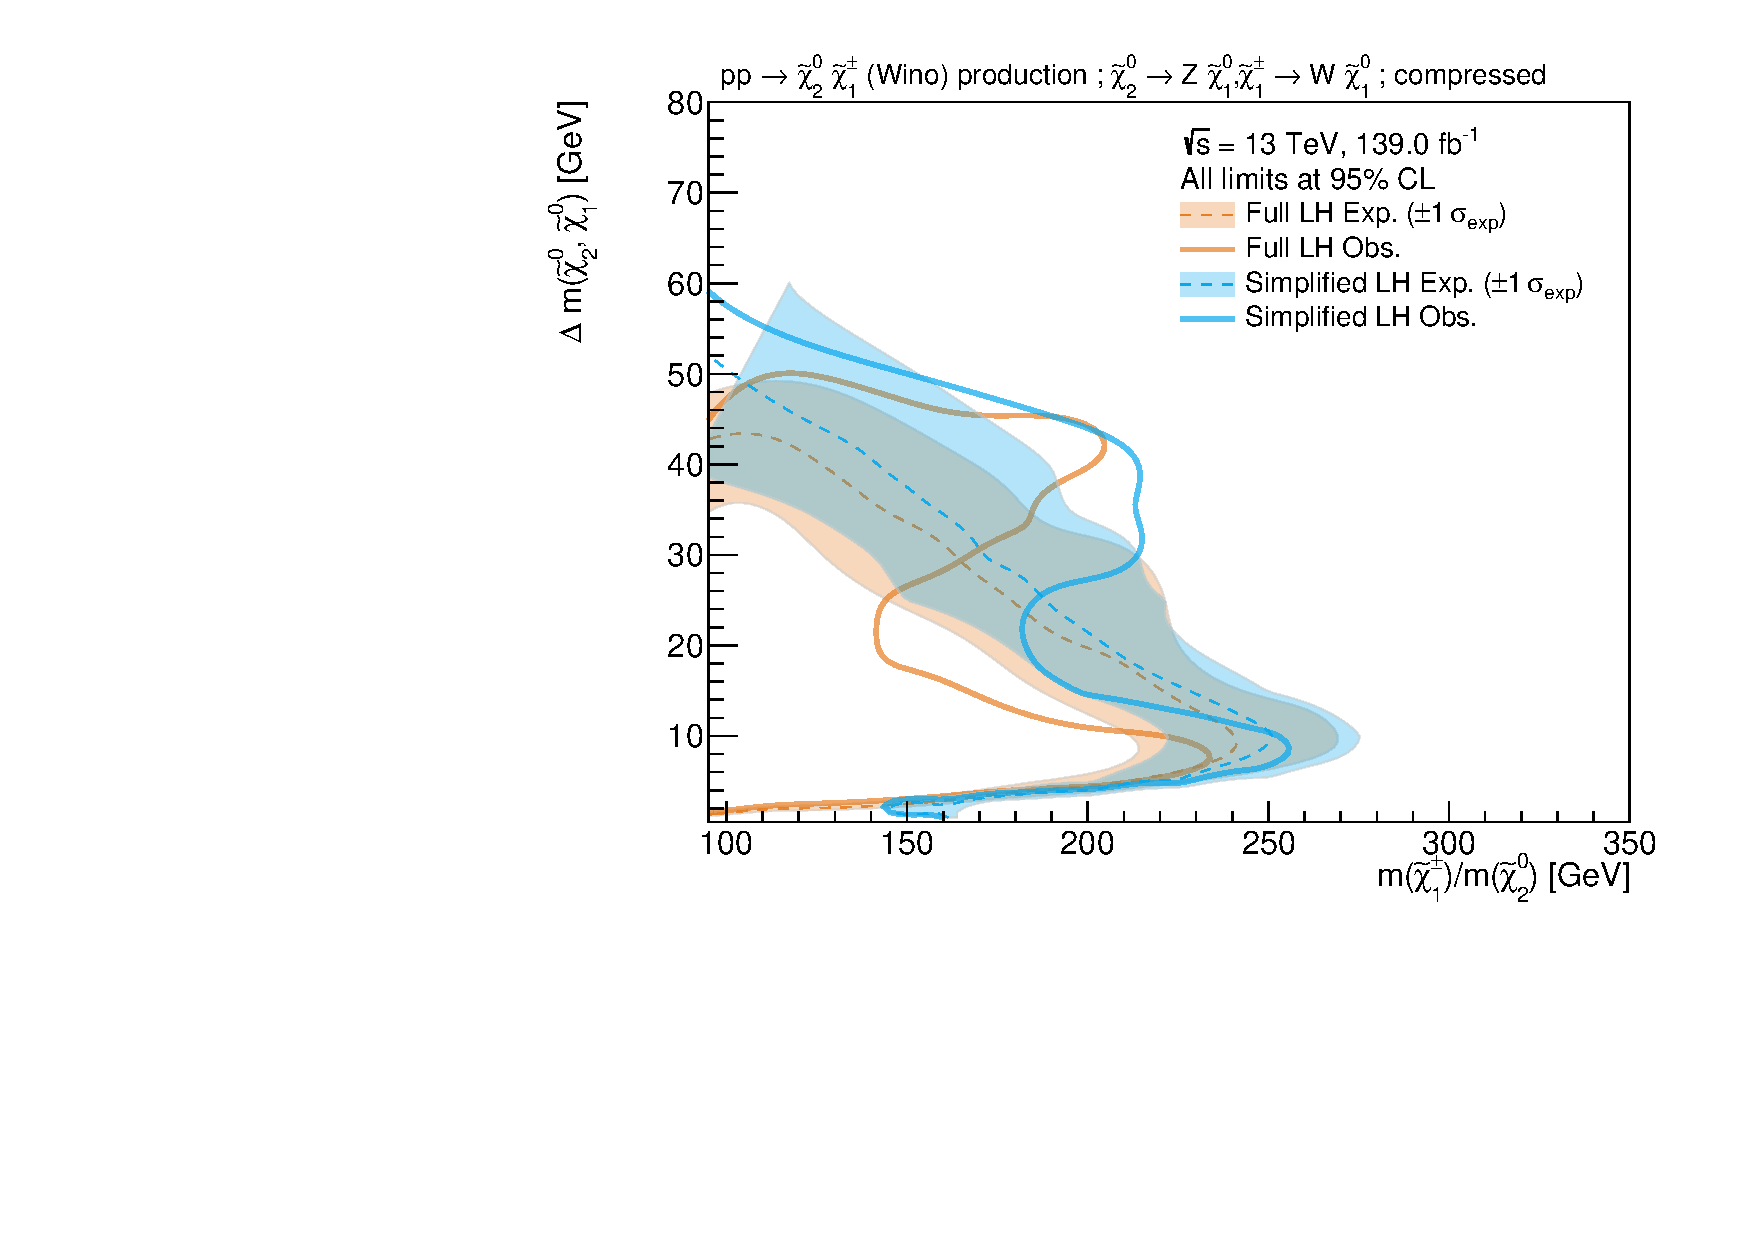
\includegraphics[width=\textwidth]{exclusion_compressed_noLabel}
		\caption{ATLAS compressed search~\cite{SUSY-2018-16}\label{fig:results_compressed}}
	\end{subfigure}\hfill
	\caption{Simplified likelihood results for the different ATLAS searches studied in this document. The results from the simplified likelihood (blue) are compared with the results of the full analysis likelihood (orange). The coloured numbers represent the observed CL$_s$ numbers obtained with both likelihoods.}\label{fig:results_analyses}
\end{figure}



\begin{figure}
	\centering
	\begin{subfigure}[b]{0.5\textwidth}
		\centering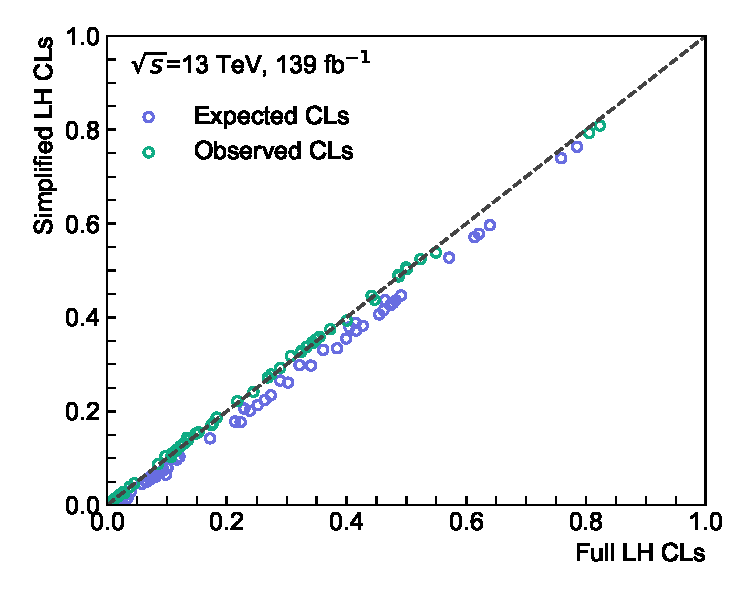
\includegraphics[width=\textwidth]{cls_scatter_sbottom_lin}
		\caption{ATLAS sbottom search~\cite{SUSY-2018-31}}
	\end{subfigure}\hfill
	\begin{subfigure}[b]{0.5\textwidth}
		\centering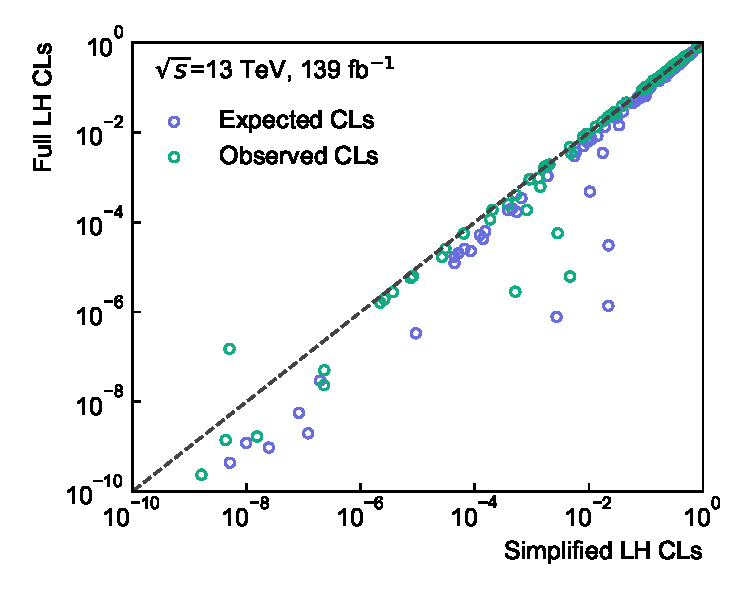
\includegraphics[width=\textwidth]{cls_scatter_sbottom_log}
		\caption{ATLAS sbottom search~\cite{SUSY-2018-31}}
	\end{subfigure}\hfill
	\begin{subfigure}[b]{0.5\textwidth}
		\centering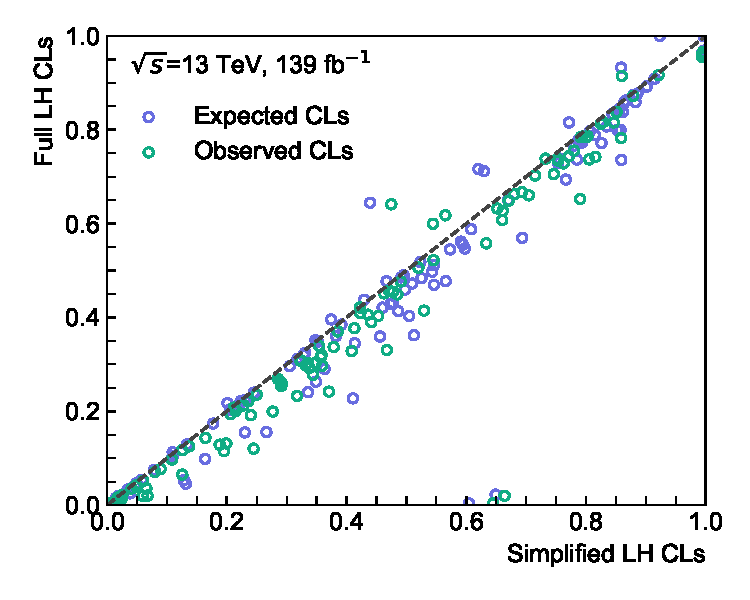
\includegraphics[width=\textwidth]{cls_scatter_stop1L_lin}
	\caption{ATLAS stop search}
	\end{subfigure}\hfill
	\begin{subfigure}[b]{0.5\textwidth}
		\centering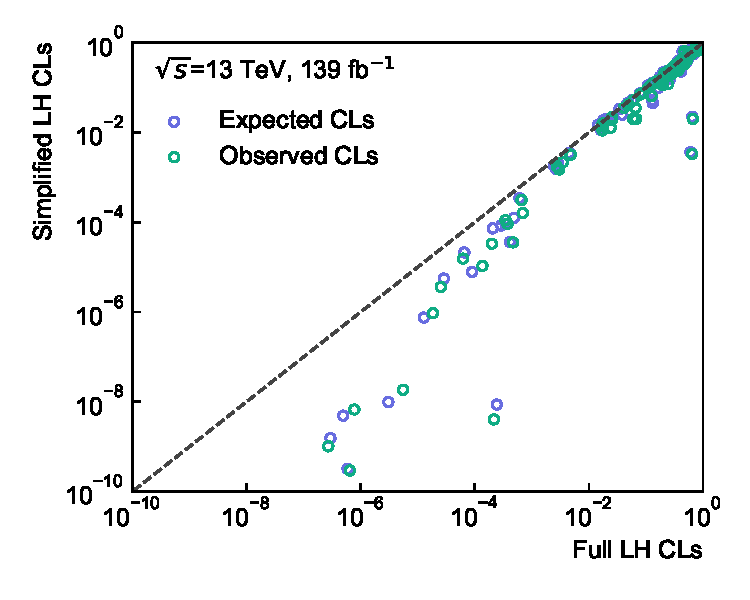
\includegraphics[width=\textwidth]{cls_scatter_stop1L_log}
		\caption{ATLAS stop search}
	\end{subfigure}\hfill
	\begin{subfigure}[b]{0.5\textwidth}
		\centering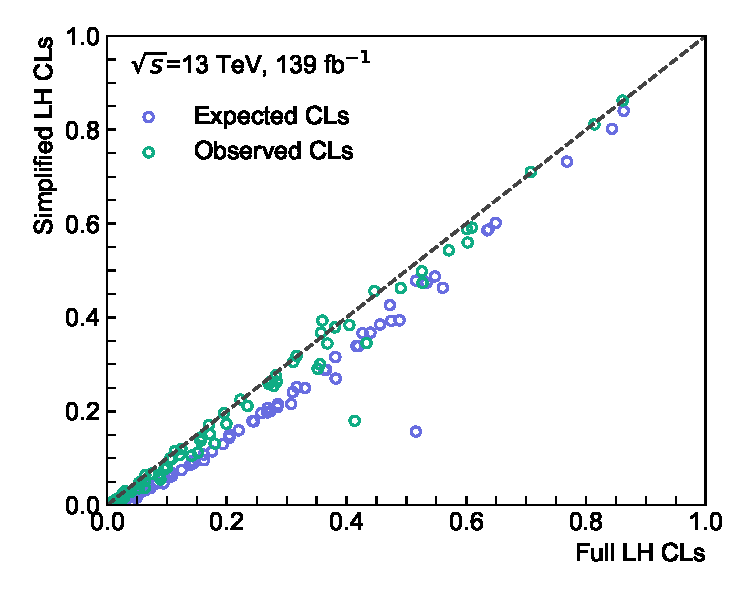
\includegraphics[width=\textwidth]{cls_scatter_2L0J_lin}
		\caption{ATLAS 2-lepton search~\cite{SUSY-2018-32}}
	\end{subfigure}\hfill
	\begin{subfigure}[b]{0.5\textwidth}
		\centering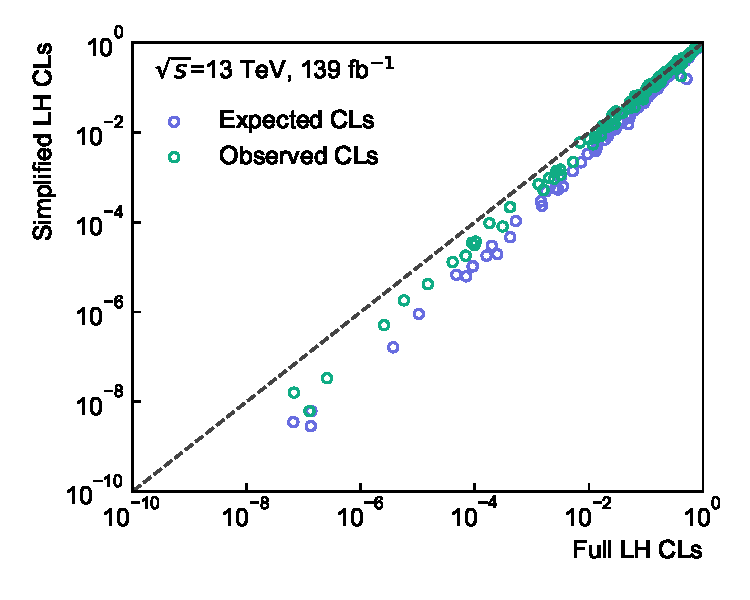
\includegraphics[width=\textwidth]{cls_scatter_2L0J_log}
		\caption{ATLAS 2-lepton search~\cite{SUSY-2018-32}}
	\end{subfigure}\hfill
	\caption{}\label{fig:app_results_cls_1}
\end{figure}


\begin{figure}
	\centering
	\begin{subfigure}[b]{0.5\textwidth}
		\centering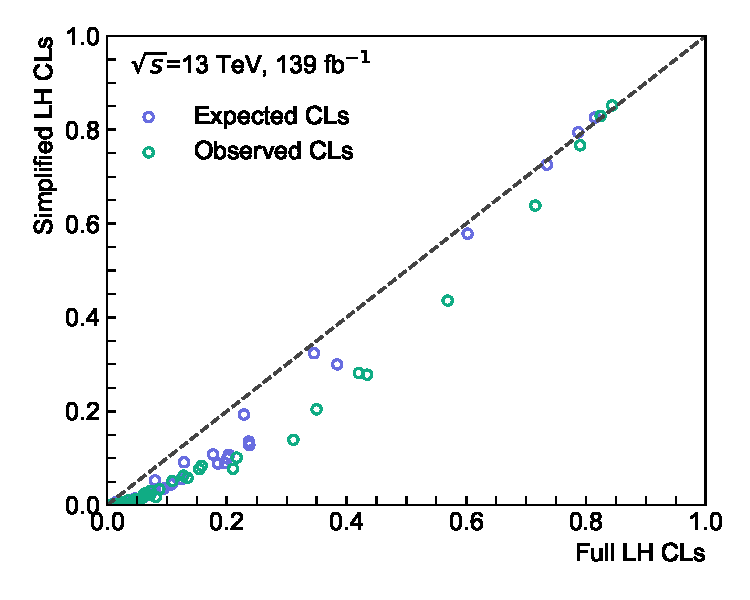
\includegraphics[width=\textwidth]{cls_scatter_directstaus_lin}
		\caption{ATLAS direct stau search~\cite{SUSY-2018-04}}
	\end{subfigure}\hfill
	\begin{subfigure}[b]{0.5\textwidth}
		\centering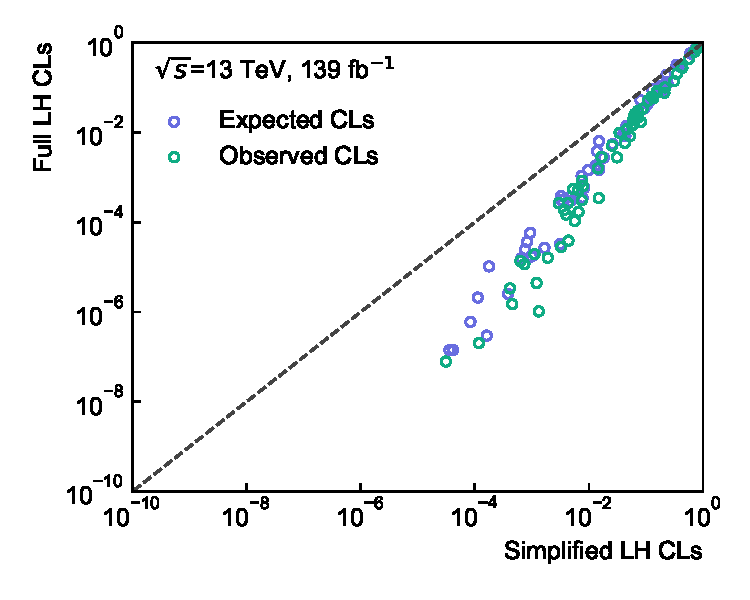
\includegraphics[width=\textwidth]{cls_scatter_directstaus_log}
		\caption{ATLAS direct stau search~\cite{SUSY-2018-04}}
	\end{subfigure}\hfill
	\begin{subfigure}[b]{0.5\textwidth}
		\centering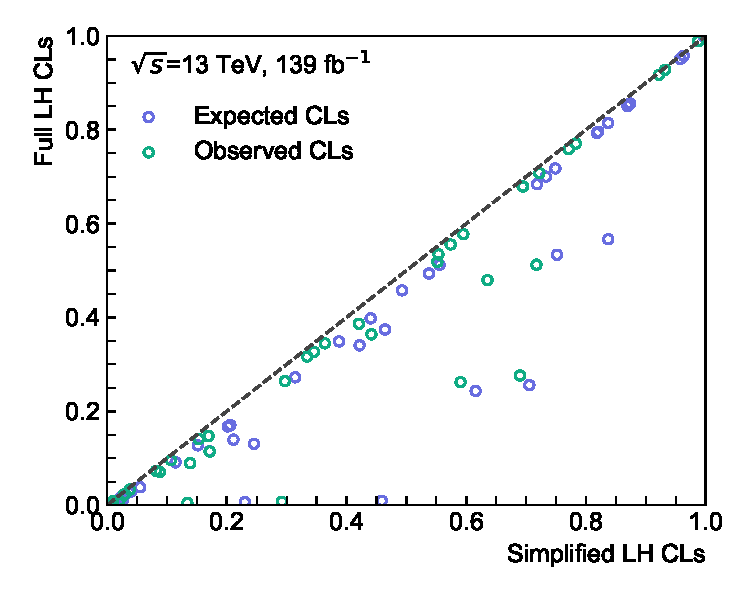
\includegraphics[width=\textwidth]{cls_scatter_3Loffshell_lin}
		\caption{ATLAS 3-lepton search}
	\end{subfigure}\hfill
	\begin{subfigure}[b]{0.5\textwidth}
		\centering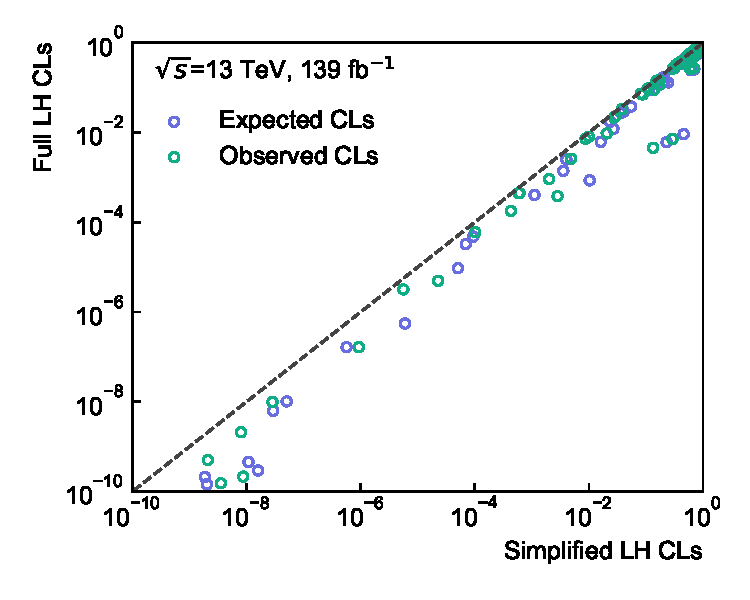
\includegraphics[width=\textwidth]{cls_scatter_3Loffshell_log}
		\caption{ATLAS 3-lepton search}
	\end{subfigure}\hfill
	\begin{subfigure}[b]{0.5\textwidth}
		\centering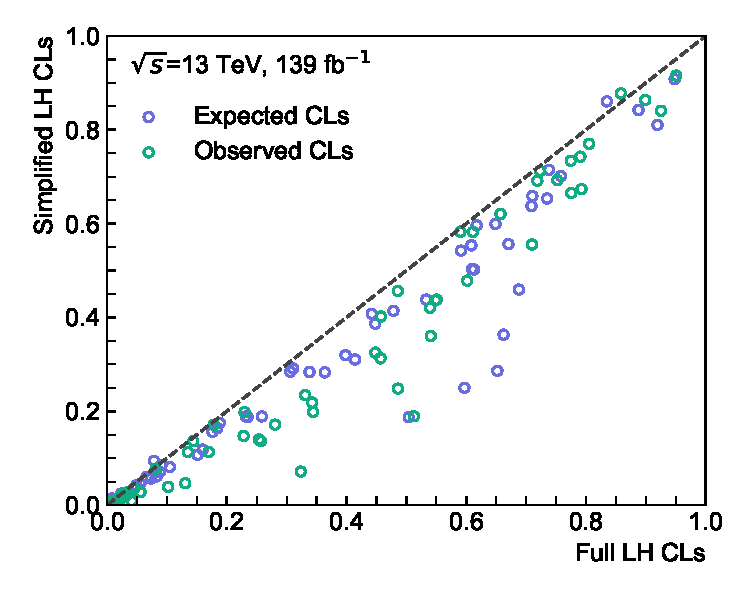
\includegraphics[width=\textwidth]{cls_scatter_compressed_lin}
		\caption{ATLAS compressed search~\cite{SUSY-2018-16}}
	\end{subfigure}\hfill
	\begin{subfigure}[b]{0.5\textwidth}
		\centering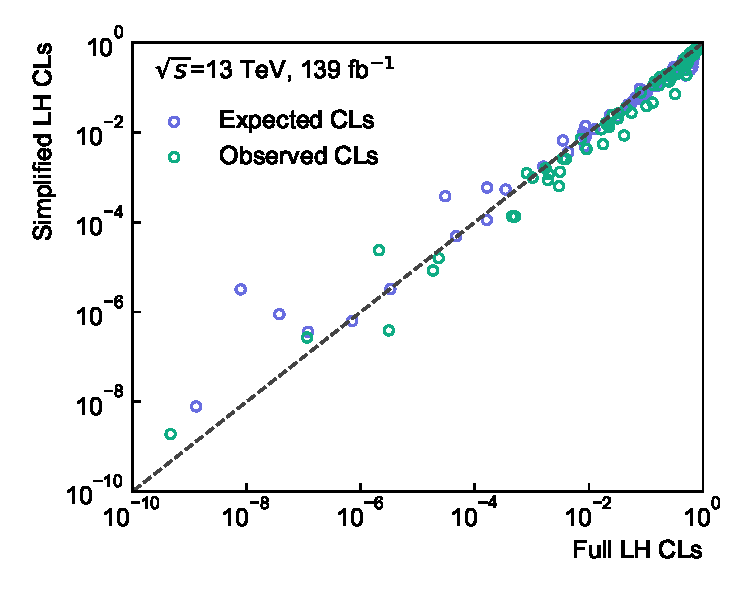
\includegraphics[width=\textwidth]{cls_scatter_compressed_log}
		\caption{ATLAS compressed search~\cite{SUSY-2018-16}}
	\end{subfigure}\hfill
	\caption{}\label{fig:app_results_cls_2}
\end{figure}